\documentclass[10pt]{elsarticle}
\usepackage{amssymb} %maths
\usepackage{amsmath} %maths
\usepackage[utf8]{inputenc} %useful to type directly diacritic characters
\usepackage{amscd}
\usepackage{amsfonts}
\usepackage{amsthm}
\usepackage{supertabular}
\usepackage{graphicx}
\usepackage{verbatim}
\usepackage{epsfig}
\usepackage{xspace}
\usepackage{euscript}
\usepackage{alltt}
\usepackage{boxedminipage}
\usepackage{float}
\usepackage{times}
\usepackage{epic}
\usepackage{eepic}
\usepackage{ifthen}
\usepackage{algorithm}
\usepackage{booktabs}
\usepackage{multirow}
\usepackage{cancel}
\usepackage{multirow}
\usepackage{array}
\usepackage{natbib}
\usepackage{appendix}

%-------------------------- macros ----------------------
%  From Alejandro's paper
\newcommand{\mbs}[1]{\boldsymbol{#1}}
\newcommand{\mbb}[1]{\mathbb{#1}}
\newcommand{\mbf}[1]{\mathbf{#1}}
\newcommand{\mbc}[1]{\boldsymbol{\mathcal{#1}}}

%\newtheorem*{proposition}{Proposition}

\def\ssst{\scriptscriptstyle}
\newcommand{\subparal}{{\ssst\|}}
\newcommand{\subperp}{{\mbox{}_{\*\bot}}}

\def\ljump{\lbrack\!\lbrack}
\def\rjump{\rbrack\!\rbrack}

\def\bA{{\mbs{A}}} \def\bB{{\mbs{B}}} \def\bC{{\mbs{C}}}
\def\bD{{\mbs{D}}} \def\bE{{\mbs{E}}} \def\bF{{\mbs{F}}}
\def\bG{{\mbs{G}}} \def\bH{{\mbs{H}}} \def\bI{{\mbs{I}}}
\def\bJ{{\mbs{J}}} \def\bK{{\mbs{K}}} \def\bL{{\mbs{L}}}
\def\bM{{\mbs{M}}} \def\bN{{\mbs{N}}} \def\bO{{\mbs{O}}}
\def\bP{{\mbs{P}}} \def\bQ{{\mbs{Q}}} \def\bR{{\mbs{R}}}
\def\bS{{\mbs{S}}} \def\bT{{\mbs{T}}} \def\bU{{\mbs{U}}}
\def\bU{{\mbs{V}}} \def\bW{{\mbs{W}}} \def\bX{{\mbs{X}}}
\def\bY{{\mbs{Y}}} \def\bZ{{\mbs{Z}}}

\def\ba{{\mbs{a}}} \def\bb{{\mbs{b}}} \def\bc{{\mbs{c}}}
\def\bd{{\mbs{d}}} \def\be{{\mbs{e}}} \def\fb{{\mbs{f}}}
\def\bg{{\mbs{g}}} \def\bh{{\mbs{h}}} \def\bi{{\mbs{i}}}
\def\bj{{\mbs{j}}} \def\bk{{\mbs{k}}} \def\bl{{\mbs{l}}}
\def\bm{{\mbs{m}}} \def\bn{{\mbs{n}}} \def\bo{{\mbs{o}}}
\def\bp{{\mbs{p}}} \def\bq{{\mbs{q}}} \def\br{{\mbs{r}}}
\def\bs{{\mbs{s}}} \def\bt{{\mbs{t}}} \def\bu{{\mbs{u}}}
\def\bv{{\mbs{v}}} \def\bw{{\mbs{w}}} \def\bx{{\mbs{x}}}
\def\by{{\mbs{y}}} \def\bz{{\mbs{z}}}

\def\balpha{{\mbs{\alpha}}}
\def\bbeta{{\mbs{\beta}}}
\def\bgamma{{\mbs{\gamma}}}
\def\bdelta{{\mbs{\delta}}}
\def\bepsilon{{\mbs{\epsilon}}}
\def\bvarepsilon{{\mbs{\varepsilon}}}
\def\bzeta{{\mbs{\zeta}}}
\def\beeta{{\mbs{\eta}}}
\def\btheta{{\mbs{\theta}}}
\def\bvartheta{{\mbs{\vartheta}}}
\def\bgamma{{\mbs{\gamma}}}
\def\bkappa{{\mbs{\kappa}}}
\def\blambda{{\mbs{\lambda}}}
\def\bmu{{\mbs{\mu}}}
\def\bnu{{\mbs{\nu}}}
\def\bxi{{\mbs{\xi}}}
\def\bomicron{{\mbs{o}}}
\def\bpi{{\mbs{\pi}}}
\def\bvarpi{{\mbs{\varpi}}}
\def\brho{{\mbs{\rho}}}
\def\bvarrho{{\mbs{\varrho}}}
\def\bsigma{{\mbs{\sigma}}}
\def\bvarsigma{{\mbs{\varsigma}}}
\def\btau{{\mbs{\tau}}}
\def\bupsilon{{\mbs{\upsilon}}}
\def\bphi{{\mbs{\phi}}}
\def\bvarphi{{\mbs{\varphi}}}
\def\bchi{{\mbs{\chi}}}
\def\bpsi{{\mbs{\psi}}}
\def\bomega{{\mbs{\omega}}}

\def\bGamma{{\mbs{\Gamma}}}
\def\bDelta{{\mbs{\Delta}}}
\def\bTheta{{\mbs{\Theta}}}
\def\bLambda{{\mbs{\Lambda}}}
\def\bXi{{\mbs{\Xi}}}
\def\bPi{{\mbs{\Pi}}}
\def\bSigma{{\mbs{\Sigma}}}
\def\bUpsilon{{\mbs{\Upsilon}}}
\def\bPhi{{\mbs{\Phi}}}
\def\bPsi{{\mbs{\Psi}}}
\def\bOmega{{\mbs{\Omega}}}

\def\dt{{\triangle t}}

\DeclareMathOperator{\tr}{tr}

\DeclareMathOperator{\divrg}{div}
\DeclareMathOperator{\grad}{grad}
\DeclareMathOperator{\curl}{curl}

\DeclareMathOperator{\Div}{Div}
\DeclareMathOperator{\Grad}{Grad}
\DeclareMathOperator{\Curl}{Curl}

\DeclareMathOperator{\dev}{dev}
\DeclareMathOperator{\vol}{vol}
\DeclareMathOperator{\Dev}{Dev}
\DeclareMathOperator{\Vol}{Vol}%
\def\bs{\boldsymbol}

\newcommand{\tensor}[1]{\ensuremath{\boldsymbol{#1}}}

\newcommand{\mathvec}[1]{\mbox{\boldmath $#1$}}
\newcommand{\labeleq}[2]{\begin{equation} \label{#1} #2 \end{equation}}
\newcommand{\rbrkt}[1]{\left(#1\right)}
\newcommand{\sbrkt}[1]{\left[#1\right]}
\newcommand{\cbrkt}[1]{\left\{#1\right\}}
\newcommand{\abrkt}[1]{\left<#1\right>}
\newcommand{\farg}[1]{\hspace{-0.2em}\rbrkt{#1}}
%\newcommand{\etal}[0]{\textit{et al.}\@ }
\newcommand{\dbyd}[2]{\frac{\partial#1}{\partial#2}}
\newcommand{\ddbydd}[3]{\frac{\partial^{2}#1}{\partial#2\partial#3}}
\newcommand{\textscript}[1]{\scriptsize{\textrm{#1}}}
\renewcommand{\thefootnote}{\fnsymbol{footnote}}
\newcommand{\paththree}{figures}
%-------------------------- macros ----------------------
\journal{International Journal of Numerical Methods in Engineering}
\begin{document}
%
\DeclareGraphicsExtensions{.pdf, .jpg, .tif, .png}
%--- graphics
\begin{frontmatter}
%
\title{Finite-deformation diffusion of hydrogen in stainless steel alloys}

\author[SNL]{J.W. Foulk III\corref{cor1}}\ead{jwfoulk@sandia.gov} \author[UC]{W. Sun}\author[NW]{G.J. Wagner}\author[SNL]{J.T. Ostien}
\author[UCB]{G.L. Bergel} \cortext[cor1]{Corresponding author}\author[SNL]{A. Mota}
\address[SNL]{Sandia National Laboratories, Livermore, CA, 94550, USA}
\address[UC]{Columbia University, New York, NY, 10027, USA}
\address[NW]{Northwestern University, Evanston, IL, 60208, USA}
\address[UCB]{University of California, Berkeley, Berkeley, CA 94720, USA}
%------------------------ abstract ----------------------
\begin{abstract}
In this work, we revisit hydrogen transport and trapping under finite deformations for both bulk and surface approaches. Consistent assumptions regarding the flux and the expression of lattice and trapping sites yield a simplified balance law in the reference configuration expressed in terms of the Cauchy-Green tensor and the Kirchhoff pressure. We illustrate the effects of deformation on transient diffusion for idealized configurations. We also develop surface element gradient operators to facilitate both deformation and transport through and along interfaces. Fast pathways for diffusion are investigated through both regular and tessellated structures. These approaches are then applied to a crack tip to illustrate the utility of the coupled methodology.\end{abstract}
%------------------------ abstract ----------------------
\begin{keyword}
hydrogen \sep transport \sep coupling \sep embrittlement
\sep finite elements
\end{keyword}
\end{frontmatter}
%
%------------------------ introduction ----------------------
%
\section{Introduction}
\label{section.introduction}
The transport of hydrogen in stainless steel alloys is of critical importance to the hydrogen economy. Past works have developed conservation laws for both hydrogen concentration \citep{Sofronis1989,Krom1998} and the equilibrium between lattice and trap sites~\cite{Oriani1970}. More recent work by Anand have 

\section{Derivation of the hydrogen transport equation}
The derivation of the transport equation stems from a model of the chemical potential and the flux. We will attempt to consider these assumptions in both the reference and current configuration. A conservation law then follows and we employ an equilibrium argument to relate the hydrogen trapped concentration to the hydrogen lattice concentration.

Given constitutive assumptions, a conservation law, and an equilibrium argument, one can derive the governing partial differential equation for hydrogen transport. We will derive the governing partial differential equation in both the reference and current configuration. We will also investigate pushing these assumptions forwards and backwards to determine the difficulty of implementation within a finite element framework.

\subsection{Constitutive model and balance law in current configuration} If we start with the chemical potential in the current configuration
\begin{equation}
\label{eq.chemical.potential}{\mu_{l} = \mu_{l}^{0} + R T \ln(\theta_{l}) - v_{h} \sigma_{h}}
\end{equation}
where $R$ is the ideal gas constant, $T$ is the temperature, $\theta_{l}$ is the site occupancy, $v_{h}$ is the partial molar volume of hydrogen, and $\sigma_{h}$ is the hydrostatic stress. The hydrostatic stress, often referred to as the pressure, is $\sigma_{h} = \frac {1} {3} \text{tr}[\bs{\sigma}]$ where $\bs{\sigma}$ is the Cauchy stress. We can express the site occupancy $\theta_{l} = c_{l}/n_{l}$ where $c_{l}$ is the hydrogen lattice concentration and $n_{l}$ is the number of lattice sites per unit volume. We seek to identify referential material constants employed in the chemical potential. Specifically, we would like to identify relations for $n_{l}$ and $v_{h}$ that preserve the number of lattice sites and the number of moles of hydrogen for a reference volume. Conservation requires $n_{l} = N_{L}/J$ and $v_{h} = V_{H}J$ where $J$ is the determinant of the deformation gradient $\bs{F} = \partial \bs{x} / \partial \bs{X}$. We then assume that the flux in the current configuration has the following form
%
\begin{equation}
\label{eq.flux}{\bs{j}_{l} = -\bs{m}_{l} c_{l} \nabla_{\bs{x}}\mu_{l}}
\end{equation}
%
with $\bs{m}_{l}$ being the mobility tensor. Defining the diffusivity tensor to be $\bs{d}_{l} = R T \bs{m}_{l} $, we can re-write the flux in light of the chemical potential to be 
%a
%\begin{equation}
%\label{eq.flux2}{\bs{j}_{l} = -\bs{d}_{l}  \nabla_{\bs{x}}c_{l} - \frac{c_{l}}{J} \bs{d}_{l} \nabla_{\bs{x}}J +\frac{c_{l}v_{h}}{R T} \bs{d}_{l} \nabla_{\bs{x}} \sigma_{h} +  \frac{c_{l}V_{H}\sigma_{h}}{RT} \bs{d}_{l} \nabla_{\bs{x}}J}
%\end{equation}
\begin{equation}
\label{eq.flux2}{\bs{j}_{l} = -\bs{d}_{l}  \nabla_{\bs{x}}c_{l} - \bigg(\frac{1}{J} \bs{d}_{l} \nabla_{\bs{x}}J -  \frac{v_{h}\sigma_{h}}{JRT} \bs{d}_{l} \nabla_{\bs{x}}J} - \frac{v_{h}}{R T} \bs{d}_{l} \nabla_{\bs{x}} \sigma_{h} \bigg)c_{l}
\end{equation}
%
where the spatial gradient of the the Jacobian is 
%
\begin{equation}
\label{eq.gradJ}{ \nabla_{\bs{x}}J} = \frac {\partial J} {\partial x_j} = J F^{-1}_{iA} \frac {\partial F_{iA}} {\partial x_j} = J F^{-1}_{iA} F_{iA,j}.
\end{equation}
which in direct form can be represented as
%
\begin{equation}
J \boldsymbol{F}^{-T}:(\nabla_{\boldsymbol{x}} \boldsymbol{F}).
\end{equation}
%
Because $\nabla_{\bs{x}}J$ contains higher order kinematics, the evaluation is not straightforward for linear elements. In fact, for the Q1/P0 element employed in this work, both the Jacobian and the pressure are constant (by construction). We can, however, obtain an approximation of the global quantities through the projection of discontinuous element fields.  For example, it is common to perform a global projection of the pressure to the nodes and then employ those nodal quantities to obtain the needed gradients at the integration points. In an attempt to simplify the pressure term in the chemical potential and avoid an additional term involving $\nabla_{\bs{x}}J$, we elect to to project $J \sigma_{h}$,  the hydrostatic component of the Kirchhoff stress $\tau_{h}$ where $\bs{\tau} = J \bs{\sigma}$.

%\begin{equation}
%\label{eq.flux3}{\bs{j}_{l} = -\bs{d}_{l}  \nabla_{\bs{x}}c_{l}  - \frac{c_{l}}{J} \bs{d}_{l} \nabla_{\bs{x}}J +  \frac{c_{l}V_{H}}{R T} \bs{d}_{l} \nabla_{\bs{x}} \tau_{h}}.
%\end{equation}
%
\begin{equation}
\label{eq.flux3}{\bs{j}_{l} = -\bs{d}_{l}  \nabla_{\bs{x}}c_{l}  - \bigg(\frac{1}{J} \bs{d}_{l} \nabla_{\bs{x}}J -  \frac{v_{h}}{JR T} \bs{d}_{l} \nabla_{\bs{x}} \tau_{h}}\bigg)c_{l}.
\end{equation}

Having developed a model for the flux, we now state a balance law for hydrogen given the total hydrogen concentration $c$ in the current configuration of the body $\mathcal{B}$
%
\begin{equation}
\label{eq.hconservation} \frac{d}{dt} \int_{\mathcal{B}} c dv = -\int_{\partial B} \bs{j} \cdot \bs{n} da 
\end{equation}
%
where $\bs{n}$ is the surface normal in the current configuration. We can then employ Reynold's transport theorem for the time derivative and arrive at 
%
\begin{equation}
\label{eq.hconservation2}  \int_{\mathcal{B}} (\dot{c} + c\text{div}\bs{v}) dv = -\int_{\partial B} \bs{j} \cdot \bs{n} da.
\end{equation}   
%
We then assert that the flux $\bs{j}$ may only derive from the flux of the lattice concentration $\bs{j}_{l}$. Using the constitutive equation model for the flux and the divergence theorem, we arrive at a local expression through a limiting process
%
%\begin{equation}
%\label{eq.hconservation3}  \int_{\mathcal{B}} \big( \dot{c} + c\text{div}\bs{v} - \nabla_{\bs{x}} \cdot \bs{d}_{l} \nabla_{\bs{x}}c_{l}   -  \nabla_{\bs{x}} \cdot \frac{c_{l}}{J} \bs{d}_{l} \nabla_{\bs{x}}J +  \nabla_{\bs{x}} \cdot  \frac{c_{l}V_{H}}{R T} \bs{d}_{l} \nabla_{\bs{x}}\tau_{h} \big) dv = 0.
%\end{equation}
%\begin{equation}
%\label{eq.hconservation3}  \int_{\mathcal{B}} \bigg( \dot{c} + c\text{div}\bs{v} - \nabla_{\bs{x}} \cdot \bs{d}_{l} \nabla_{\bs{x}}c_{l}   -  \nabla_{\bs{x}} \cdot \bigg[ \frac{1}{J} \bs{d}_{l} %\nabla_{\bs{x}}J -  \frac{v_{h}}{JR T} \bs{d}_{l} \nabla_{\bs{x}}\tau_{h}\bigg] c_{l} \bigg) dv = 0.
%\end{equation}
\begin{equation}
\label{eq.hconservation3}  \dot{c} + c\text{div}\bs{v} - \nabla_{\bs{x}} \cdot \bs{d}_{l} \nabla_{\bs{x}}c_{l}   -  \nabla_{\bs{x}} \cdot \bigg[ \frac{1}{J} \bs{d}_{l} \nabla_{\bs{x}}J -  \frac{v_{h}}{JR T} \bs{d}_{l} \nabla_{\bs{x}}\tau_{h}\bigg] c_{l}  =  0.
\end{equation}
%
In order to move forward, we need to partition the hydrogen concentration $c$ into lattice and trapped components $c = c_{l} + c_{t}$. Using an the equilibrium assumption of Oriani \cite{Oriani1970}, we can specify $c_{t}$ in terms of the occupancy
%
\begin{equation}
\label{eq.oriani1} \theta_{t} = \frac{1}{1 + \frac{1}{k_{t} \theta_{l}}}.
\end{equation}
where $k_t$ is the trap equilibrium constant $k_{t} = \exp[(\mu^{0}_{l} - \mu^{0}_{t})/RT]$ .  We note that the equilibrium relation noted in Equation~\ref{eq.oriani1} derives from a chemical potential that must also incorporate the hydrostatic stress, $\mu_{t} =  \mu_{t}^{0} + RT\ln[\theta_{t}/(1-\theta_{t})] - \nu_{h}\sigma_{h} $. Given that $\theta_{l} = c_{l}/n_{l}$ and $\theta_{t} = c_{t}/n_{t}$, we can re-write the equilibrium of $c_{t}$ in terms of $c_{l}$ and $n_{t}$. 
%
\begin{equation}
\label{eq.oriani2} c_{t} = \frac{n_{t}}{1 + \frac{n_{l}}{k_{t} c_{l}}}
\end{equation}
As an initial model for trapping, we assume that the number of trapped sites $n_{t}$ is a function of the permanent deformation of the body through the equivalent plastic strain $\epsilon_{p}$. To conserve the number of trap sites under elastic changes in volume, we specify $n_{t} = N_{T}(\epsilon_{p})/J$ where $N_{T}$ is referential quantity.  It follows that
%
\begin{equation}
\label{eq.cdot2}{\dot{c} = \dot{c}_{l} + \frac{\partial c_{t}}{\partial c_{l}} \dot{c}_{l} + \frac{\partial c_{t}}{\partial n_{t}} \frac{\partial n_{t}}{\partial \epsilon_{p}} \dot{\epsilon}_{p}} +  \frac{\partial c_{t}}{\partial n_{t}} \frac{\partial n_{t}}{\partial J} \dot{J}
\end{equation}
%
which can be simplified to
%
\begin{equation}
\label{eq.cdot}{\dot{c} = \dot{c}_{l} + \frac{\partial c_{t}}{\partial c_{l}} \dot{c}_{l} + \frac{\theta_{l}}{J} \frac{\partial N_{T}}{\partial \epsilon_{p}} \dot{\epsilon}_{p} -  \frac{\theta_{t} N_{T}}{J^{2}}  \dot{J}}.
\end{equation}
%
We can then use obtain a revised expression for the conservation of hydrogen
\begin{align}
\label{eq.hconservation4}  
%\int_{\mathcal{B}} (D^{*}\dot{c}_{l} + C^{*}\text{div}\bs{v} - \nabla_{\bs{x}} \cdot \bs{d}_{l} \nabla_{\bs{x}}c_{l}   -  \nabla_{\bs{x}} \cdot \frac{c_{l}}{J} \bs{d}_{l} \nabla_{\bs{x}}J +  \nabla_{\bs{x}} \cdot  \frac{c_{l}V_{H}}{R T} \bs{d}_{l} \nabla_{\bs{x}}\sigma_{h}  +  \nonumber \\ \frac{\theta_{l}}{J} \frac{\partial N_{T}}{\partial \epsilon_{p}} \dot{\epsilon}_{p} -  \frac{\theta_{t} N_{T}}{J^{2}}  \dot{J} )dv = 0.
% \int_{\mathcal{B}} (D^{*}\dot{c}_{l} + C^{*}\text{div}\bs{v} - \nabla_{\bs{x}} \cdot \bs{d}_{l} \nabla_{\bs{x}}c_{l}   -  \nabla_{\bs{x}} \cdot \bigg[ \frac{1}{J} \bs{d}_{l} \nabla_{\bs{x}}J -  \frac{V_{H}}{R T} \bs{d}_{l} \nabla_{\bs{x}}\tau_{h}\bigg] c_{l}  +  \nonumber \\ \frac{\theta_{l}}{J} \frac{\partial N_{T}}{\partial \epsilon_{p}} \dot{\epsilon}_{p} -  \frac{\theta_{t} N_{T}}{J^{2}}  \dot{J} )dv = 0.
 D^{*}\dot{c}_{l} + C^{*}\text{div}\bs{v} - \nabla_{\bs{x}} \cdot \bs{d}_{l} \nabla_{\bs{x}}c_{l}   -  \nabla_{\bs{x}} \cdot \bigg[ \frac{1}{J} \bs{d}_{l} \nabla_{\bs{x}}J -  \frac{V_{H}}{R T} \bs{d}_{l} \nabla_{\bs{x}}\tau_{h}\bigg] c_{l}  +  \nonumber \\ \frac{\theta_{l}}{J} \frac{\partial N_{T}}{\partial \epsilon_{p}} \dot{\epsilon}_{p} -  \frac{\theta_{t} N_{T}}{J^{2}}  \dot{J} = 0
\end{align}
where $D^{*}$ and $C^{*}$ and $\theta_{t}$ are defined to be independent of $c_{t}$ through
%
\begin{equation}
\label{eq.Dstar}{D^{*} = 1 + \frac{\partial c_{t}}{\partial c_{l}} = 1 + \frac{n_{t} n_{l}}{k_{t} c_{l}^{2}}\bigg[ \frac{1}{(1+ \frac{n_{l}}{k_{t} c_{l}})^{2}}\bigg] }
\end{equation}
%
\begin{equation}
\label{eq.Cstar}{C^{*} = c_{l} +\frac{n_{t}}{1 + \frac{n_{l}}{k_{t} c_{l}}} }
\end{equation}
%
\begin{equation}
\label{eq.thetat2}{\theta_{t} = \frac{1}{1 + \frac{n_{l}}{k_{t} c_{l}}} }.
\end{equation}
%
%Assuming a limiting process, we can obtain a strong form of the partial differential equation for hydrogen transport.
%
%\begin{align}
%\label{eq.hconservation5}  D^{*}\dot{c}_{l} + C^{*}\text{div}\bs{v} - \nabla_{\bs{x}} \cdot \bs{d}_{l} \nabla_{\bs{x}}c_{l} -  \nabla_{\bs{x}} \cdot \frac{c_{l}}{J} \bs{d}_{l} \nabla_{\bs{x}}J  +  \nabla_{\bs{x}} \cdot  \frac{c_{l}V_{H}}{R T} \bs{d}_{l}\nabla_{\bs{x}}\tau_{h}  + \nonumber \\  \frac{\theta_{l}}{J} \frac{\partial N_{T}}{\partial \epsilon_{p}} \dot{\epsilon}_{p} -  \frac{\theta_{t} N_{T}}{J^{2}}  \dot{J} = 0
%\end{align}
%
%Given the partial differential equation, we can also construct a weak form with a test function $v$.  After multiplying by a test function and employing integration by parts and the properties of the test function ($v = 0$ on $\partial B_{c}$), the weak form yields
%
%\begin{eqnarray}
%\label{eq.weakform}  \int_{\mathcal{B}}  (D^{*}\dot{c}_{l} + C^{*}\text{div}\bs{v} + \frac{\theta_{l}}{J} \frac{\partial N_{T}}{\partial \epsilon_{p}} \dot{\epsilon}_{p} -  \frac{\theta_{t} N_{T}}{J^{2}}  \dot{J})vdv + \int_{\mathcal{B}} \bs{d}_{l} \nabla_{\bs{x}}c_{l} \cdot  \nabla_{\bs{x}}vdv + \nonumber \\  \int_{\mathcal{B}} \frac{c_{l}}{J} \bs{d}_{l} \nabla_{\bs{x}}J  \cdot  \nabla_{\bs{x}}vdv - \int_{\mathcal{B}} \frac{c_{l}V_{H}}{R T} \bs{d}_{l} \nabla_{\bs{x}}\tau_{h} \cdot \nabla_{\bs{x}}v dv + \int_{\partial B_{\Gamma}} (\bs{j} \cdot \bs{n}) v da = 0.
%\label{eq.weakform}  \int_{\mathcal{B}}  \bigg( D^{*}\dot{c}_{l} + C^{*}\text{div}\bs{v} + \frac{\theta_{l}}{J} \frac{\partial N_{T}}{\partial \epsilon_{p}} \dot{\epsilon}_{p} -  \frac{\theta_{t} N_{T}}{J^{2}}  \dot{J} \bigg)vdv + \int_{\mathcal{B}} \bs{d}_{l} \nabla_{\bs{x}}c_{l} \cdot  \nabla_{\bs{x}}vdv + \nonumber \\  \int_{\mathcal{B}} \bigg( \frac{1}{J} \bs{d}_{l} \nabla_{\bs{x}}J - \frac{V_{H}}{R T} \bs{d}_{l} \nabla_{\bs{x}}\tau_{h} \bigg)c_{l}   \cdot  \nabla_{\bs{x}}vdv + \int_{\partial B_{\Gamma}} (\bs{j}_{app} \cdot \bs{n}) v da = 0.
%\end{eqnarray}
This form of the transport equation is found in the literature but often authors do not distinguish between $v_{h}$, $n_{l}$ and $n_{t}$, and $V_{H}$, $N_{L}$, and $N_{T}$. The inclusion of reference quantities (and their corresponding conservation equations) yields additional terms involving $\nabla_{\bs{x}}J$ and $\dot{J}$.  We also note that in many works, the authors assume that $div\bs{v} = 0$.  

\subsection{Simplification through the reference configuration}
In an effort to simplify both the formulation and the implementation, we consider a push back to the reference configuration. Given that $J$ is a nonlinear kinematic quantity, we seek to avoid errors in the approximation of space $\nabla_{\bs{x}}J$ and time  $\dot{J}$. We begin with the conservation equation that has been pushed back to the reference configuration
%
\begin{equation}
\label{eq.hconservationref} \frac{d}{dt} \int_{\mathcal{B}_{0}} C dV = -\int_{\partial B_{0}} J\bs{F}^{-1}\bs{j} \cdot \bs{N} dA 
\end{equation}
where $C$ is the hydrogen concentration in the reference configuration and $C = Jc$. The chemical potential is still written in the current configuration but the concentration $c_{l}$, number of lattice sites $n_{l}$, and molar volume $v_{h}$ are all expressed as referential quantities $C_{L}$, $N_{L}$, and $V_{H}$, respectively.
%
\begin{equation}
\label{eq.chemical.potential}{\mu_{l} = \mu^{0}_{l} + R T \ln \bigg( \frac{C_{L}}{N_{L}} \bigg) - J V_{h} \sigma_{h}}.
\end{equation}
%
As before, the pressure contribution to the chemical potential is simplified through the Kirchhoff stress tensor $\tau_{h} = J\sigma_{h}$ and the diffusivity is written in terms of the mobility. We relate the spatial gradient to referential gradient through $\nabla_{\bs{x}} = \bs{F}^{-T}\nabla_{\bs{X}}$ and find the flux to be 
%
%\begin{equation}
%\label{eq.flux.ref}{\bs{j}_{l} = -\bs{m}_{l} c_{l} \nabla_{\bs{x}}\mu_{l}} =  -\frac{R T}{J}\bs{m}_{l}  \nabla_{\bs{x}}C_{L}  + \frac{ V_{H}}{J} \bs{m}_{l}  \nabla_{\bs{x}}\tau_{h}C_{L}.
%\end{equation}
%
%If we employ the diffusivity $\bs{d}_{l} = RT \bs{m}_{l}$, and $\nabla_{\bs{x}} = \bs{F}^{-T}\nabla_{\bs{X}}$, we find that the flux to be
%
\begin{equation}
\label{eq.flux.ref3}{\bs{j}_{l} = -\frac{1}{J} \bs{d}_{l} \bs{F}^{-T} \nabla_{\bs{X}}C_{L}  + \frac{V_{H}}{J R T} \bs{d}_{l}  \bs{F}^{-T} \nabla_{\bs{X}} \tau_{h}} C
_{L}.
\end{equation}
Employing the model of the flux along with the divergence theorem and a limiting process, we find 
%
%\begin{align}
%\label{eq.hconservationref2} \frac{d}{dt} \int_{\mathcal{B}_{0}} C dV =  \nonumber \\ \int_{\partial B_{0}} \bigg( \bs{F}^{-1} \bs{d}_{l}   \bs{F}^{-T}  \nabla_{\bs{X}} C_{L} -  \frac{V_{H}}{RT} \bs{F}^{-1} \bs{d}_{l}   \bs{F}^{-T}  \nabla_{\bs{X}}\tau_{h} C_{L} \bigg) \cdot \bs{N} dA 
%\end{align}
%
%and further simplify the relations through either a reference diffusivity tensor $\bs{D}_{L} = \bs{F}^{-1} \bs{d}_{l}   \bs{F}^{-T}$ or invoking isotropy $\bs{d}_{l} = d_{l}\bs{I}$. %Because the materials in question are cubic and isotropic, we invoke isotropy and the divergence theorem to yield
%
%\begin{equation}
%\label{eq.hconservationref2} \frac{d}{dt} \int_{\mathcal{B}_{0}} C dV =  \\ \int_{\partial B_{0}} \bigg(d_{l} \bs{C}^{-1}  \nabla_{\bs{X}} C_{L} -  \frac{ d_{l} C_{L}V_{H}}{RT} \bs{C}^{-1} \nabla_{\bs{X}} \tau_{h} \bigg) \cdot \bs{N} dA 
%\end{equation}
%where $\bs{C}$ is the right-hand Cauchy-Green tensor $\bs{C} = \bs{F}^{T}\bs{F}$. Employing the divergence theorem we have
%
%\begin{equation}
%\label{eq.hconservationref3} \int_{\mathcal{B}_{0}} \bigg( \dot{C} -   \nabla_{\bs{X}}  \cdot d_{l} \bs{C}^{-1}  \nabla_{\bs{X}} C_{L}  +   \nabla_{\bs{X}}  \cdot \frac{ d_{l} V_{H}}{RT} \bs{C}^{-1} \nabla_{\bs{X}} \tau_{h} C_{L} \bigg) dV = 0.
%\end{equation}
%
\begin{equation}
\label{eq.hconservationref3} \dot{C} -   \nabla_{\bs{X}}  \cdot \bs{D}_{L}  \nabla_{\bs{X}} C_{L}  +   \nabla_{\bs{X}}  \cdot \frac{V_{H}}{RT} \bs{D}_{L}  \nabla_{\bs{X}} \tau_{h} C_{L}  = 0
\end{equation}
where $\bs{D}_{L} = \bs{F}^{-1} \bs{d}_{l}   \bs{F}^{-T}$. We can now re-examine the time derivatives in terms of the reference configuration. We can express the number lattice sites in terms of $N_{L}$ and the evolving trap sites as $N_{T} = N_{T}(\epsilon_{p})$. Through $\theta_{L} = C_{L}/N_{L}$ and $\theta_{T} = C_{T}/N_{T}$, we find a simplification
%
\begin{equation}
\label{eq.cdotref}{\dot{C} = \dot{C}_{L} + \frac{\partial C_{T}}{\partial C_{L}} \dot{C}_{L} +\theta_{T} \frac{d N_{T}}{d \epsilon_{p}} \dot{\epsilon}_{p}} 
\end{equation}
and plug those relations into the conservation equation
%
\begin{align}
\label{eq.hconservationref4} \int_{\mathcal{B}_{0}} \bigg( D^{*}\dot{C_{L}} -   \nabla_{\bs{X}}  \cdot d_{l} \bs{C}^{-1}  \nabla_{\bs{X}} C_{L}  +   \nonumber \\ \nabla_{\bs{X}}  \cdot \frac{d_{l} V_{H}}{RT} \bs{C}^{-1} \nabla_{\bs{X}} \tau_{h} C_{L} + \theta_{T} \frac{d N_{T}}{d \epsilon_{p}} \dot{\epsilon}_{p} \bigg) dV = 0.
\end{align}
where $D^{*} = 1 + \partial C_{T}/ \partial C_{L}$. We can identify referential relations for $\theta_{T}$, $C_{T}$, and $D^{*}$  that mirror Equations \ref{eq.oriani1}, \ref{eq.oriani2}, and \ref{eq.Dstar}, respectively. In parallel with the current configuration, we can develop a weak form of the transport equation
%
\begin{align}
\label{eq.hconservationref5} \int_{B_{0}} \bigg( D^{*}\dot{C_{L}} +  \theta_{T} \frac{d N_{T}}{d \epsilon_{p}} \dot{\epsilon}_{p} \bigg)vdV  + \int_{B_{0}}  d_{l} \bs{C}^{-1}  \nabla_{\bs{X}} C_{L}  \cdot  \nabla_{\bs{X}}v dV - \nonumber \\ \int_{B_{0}}  \frac{d_{l} V_{H}}{RT} \bs{C}^{-1} \nabla_{\bs{X}} \tau_{h}C_{L}  \cdot \nabla_{\bs{X}}v dV + \int_{\partial \Gamma_{0}} J\bs{F}^{-1}\bs{j}_{app} \cdot \bs{N}vdA = 0
\end{align}
%
where the applied flux in the current configuration $\bs{j}_{app}$ is pushed back to the reference configuration. We note that we note that the weak form the the reference configuration avoids the need to evaluate third-order tensors and greatly simplifies the implementation. 
%We can now consider a limiting process to find the partial differential equation
%
%\begin{equation}
%\label{eq.hconservationref5} D^{*}\dot{C_{L}} -   \nabla_{\bs{X}}  \cdot d_{l} \bs{C}^{-1}  \nabla_{\bs{X}} C_{L} +    \nabla_{\bs{X}}  \cdot \frac{d_{l} C_{L}V_{H}}{RT} \bs{C}^{-1} \nabla_{\bs{X}}\tau_{h} + \theta_{T} \frac{d N_{T}}{d \epsilon_{p}} \dot{\epsilon}_{p} = 0
%\end{equation}
%where the equilibrium relations are 
%
%\begin{equation}
%\label{eq.thetat.ref} \theta_{T} = \frac{1}{1 + \frac{N_{L}}{k_{t} C_{L}}}
%\end{equation}
%
%and
%
%\begin{equation}
%\label{eq.oriani2ref} C_{T} = \frac{N_{T}}{1 + \frac{N_{L}}{k_{t} C_{L}}}
%\end{equation}
%
%and $D^{*}$ is
%
%\begin{equation}
%\label{eq.Dstar.ref}D^{*} = 1 + \frac{\partial C_{T}}{\partial C_{L}} = 1 + \frac{N_{T} N_{L}}{k_{t} C_{L}^{2}}\bigg[ \frac{1}{(1+ \frac{N_{L}}{k_{t} C_{L}})^{2}}\bigg] = 1 + \frac{N_{T} N_{L}}{k_{t}C_{L}^{2}} \theta_{T}^{2}.
%\end{equation}

Notice that in the term 
$\nabla_{\bs{X}}  \cdot \frac{d_{l} C_{L}V_{H}}{RT} \bs{C}^{-1} \nabla_{\bs{X}}\tau_{h}$ \eqref{eq.hconservationref5}
requires one to evaluate the gradient of hydrostatic stress $\tau_{h}$. In a typical finite element model
(except the nodal integration method \cite{Krysl:2008}), physical quantities such as deformation gradient
 and stress are typically only evaluated at the integration points but not at the nodal points. 
 Consequently, the hydrostatic stress field must be extrapolated as a $C^{o}$ field  such that the gradient of the hydrostatic
 stress can be computed properly. Here we employ a global $L_{2}$ projection scheme to recover the gradient field. 
 
Finally, the fully coupled convection-diffusion-deformation coupling problem is completed upon augmenting the hydrogen transport equation with the balance of linear momentum, i.e.,
\begin{equation}
\label{eq:balanceLinearMomentum} \Div \tensor{P} +  \bB = \b0  
\end{equation}
where $\tensor{P}$ is the first Piola-Kirchhoff stress and $\bB$ is the body force. 
%

\subsection{Implementation in reference configuration}
The weak form of the fully coupled convection-diffusion-deformation coupling problems is constructed
through the weighted residual method. In the weak statement, there are three unknown variables to be solved, i.e. 
the displacement $\bu$, the hydrogen lattice concentration $C_{L}$  and the projected hydrostatic stress $\hat{\tau_{h}}$. 
The corresponding trial space therefore reads, 
\begin{eqnarray}
    \label{eq:trialSpace}
      V_{\bu} &=& \{ \bu : \mathcal{B} \rightarrow \mathbb{R}^{3} | \bu \in [H^{1}(\mathcal{B})]^{3} , \label{eq:uspace} \bu|_{\partial B_{\bu}} = \overline{\bu} \} \nonumber \\
       V_{C_{L}} &=& \{ C_{L} : \mathcal{B} \rightarrow \mathbb{R} | C_{L} \in H^{1}(\mathcal{B}), C_{L}|_{\partial B_{C_{L}}} = \overline{C_{L}} \} \\
      V_{\hat{\tau_{h}}} &=& \{  \hat{\tau_{h}} : \mathcal{B} \rightarrow \mathbb{R} | \hat{\tau_{h}} \in H^{1}(\mathcal{B}) \} \nonumber 
    \end{eqnarray}
    where $H^{1}$ denotes the Sobolev space of degree one.  The
    admissible space for the weighting functions of displacement $\beeta$, hydrogen lattice concentration $v$ and projected hydrostatic pressure $\psi$ therefore read,
    \begin{eqnarray}
    \label{eq:variation}
      V_{\beeta} &=& \{  \beeta : \mathcal{B} \rightarrow \mathbb{R}^{3} | \beta \in [H^{1}(\mathcal{B})]^{3} ,  \beeta|_{\partial B_{\beeta}} = \b0 \} \nonumber \\
      V_{v} &=& \{ v : \mathcal{B} \rightarrow \mathbb{R} | v \in H^{1}(\mathcal{B}), v|_{\partial B_{C_{L}}} =0 \}  \\
      V_{\psi} &=& \{ \psi : \mathcal{B} \rightarrow \mathbb{R} | \psi \in H^{1}(\mathcal{B}) \}
      \nonumber 
      \label{eq:varp}
    \end{eqnarray}
    For brevity, the spatial argument $\vec{X} \in \mathcal{B}$ is not
    explicitly written. After multiplying by the test function and employing integration by parts, the weak statement can be written as follows. 
    
Find $\bu \in V_{\bu}$, $C_{L} \in V_{C_{L}}$ and $\hat{\tau}_{h} \in V_{\hat{\tau}_{h}}$ such that for all variations
 $\beeta \in V_{\beeta}$, $v \in V_{v}$ and $\psi = V_{\psi}$, the following statements hold,      
\begin{equation}
\label{eq.weakBalanceLinearMomentum}
\int_{\mathcal{B}_{0}}   \tensor{P}  \cdot \nabla_{\bs{X}}  \beeta + \bB  \cdot \beeta dV  - \int_{\partial \Gamma_{0}}   \bt  \cdot \beeta \; dA = 0
\end{equation}    
\begin{align}
\label{eq.hconservationref5_1} \int_{\mathcal{B}_{0}} \bigg[ \big( D^{*}\dot{C_{L}} +  \theta_{T} \frac{d N_{T}}{d \epsilon_{p}} \dot{\epsilon}_{p} \big)v  +   d_{l} \bs{C}^{-1}  \nabla_{\bs{X}} C_{L}  \cdot  \nabla_{\bs{X}}v  - \nonumber \\ \frac{d_{l} C_{L}V_{H}}{RT} \bs{C}^{-1} \nabla_{\bs{X}} \hat{\tau}_{h}  \cdot \nabla_{\bs{X}}v \bigg] dV + \int_{\partial \Gamma_{0}} J\bs{F}^{-1}\bs{j}_{app} \cdot \bs{N}v \; dA = 0
\end{align}
\begin{equation}
\label{eq.weakL2Proj} \int_{\mathcal{B}} \Big( \tau_{h} - \hat{\tau_{h}} \Big) \psi \; dV = 0
\end{equation}

We note that although the weak form expressed in \eqref{eq.hconservationref5} is formulated in the reference configuration, both the flux and the balance law were pushed back from the current configuration . This enables consistency in the application of the flux boundary condition. The weak form enables a natural push-back of $j_{app}$. Furthermore, notice that the term that depends 
on the gradient of the hydrostatic stress $\nabla_{\bs{X}} \tau_{h}$is now depending on the gradient of the  projected hydrostatic stress $\nabla_{\bs{X}} \hat{\tau}_{h}$, which can be easily computed via the basis function and the nodal values. 
From \eqref{eq.weakL2Proj} is the weak form that leads to a $L_{2}$ global projection (cf. \citep{Mota:2013}).

Moreover, it is trivial to see that one can obtain the Galerkin form of the fully coupled problem by
 using finite dimensional spaces as the trial and variation spaces of the unknown variables.
To simplify the implementation and avoid using multiple meshes, 
we use the trial and  weighting space of all unknown variables that are spanned by the same basis functions. 
The resultant finite dimensional trial and weighting spaces for $\bu$, $C_{L}$ and $\hat{\tau}_{h}$  therefore reads, 
\begin{eqnarray}
    \label{eq.DisTrialSpaceAndVariation}
      V_{\bu}^{h} &=& \{ \bu = \sum_{a=1}^{n_{np}} N_{a} \bu_{a}  \bu|_{\partial B_{\bu}} = \overline{\bu} \} \nonumber \\
       V_{C_{L}}^{h} &=& \{ C_{L} = \sum_{a=1}^{n_{np}} N_{a} C_{La} |  C_{L}|_{\partial B_{C_{L}}} = \overline{C_{L}} \} \\
      V_{\hat{\tau_{h}}}^{h} &=& \{ \hat{\tau}_{h} =  \sum_{a=1}^{n_{np}} N_{a}  \hat{\tau}_{ha} \} \nonumber \\
    \label{eq.DisVariation}
      V_{\beeta}^{h} &=& \{ \beeta = \sum_{a=1}^{n_{np}} N_{a} \beeta_{a}  \bu|_{\partial B_{\bu}} = \b0 \} \nonumber \\
      V_{v}^{h} &=& \{ v = \sum_{a=1}^{n_{np}} N_{a} v_{a} |  v|_{\partial B_{C_{L}}} = 0 \} \\
      V_{\psi}^{h} &=& \{ \psi =  \sum_{a=1}^{n_{np}} N_{a}  \psi_{a} \} \nonumber 
      \nonumber 
      \label{eq:varp}
    \end{eqnarray}
where $n_{np}$ denotes the number of nodal points per element.     

\subsection{Pressure-dependent essential boundary conditions}
For the undeformed case, the application of essential, concentration boundary conditions is straightforward. As pointed out by numerous authors \cite{Wriedt1970,SanMarchi2007,Anand2013}, the applied concentration must evolve on the boundary to enforce a constant chemical equilibrium between the gas and the stressed solid. We refer the reader to \citet{Anand2013} for studies that examine an evolving concentration. In this presentation, we parallel the presentation of \citet{SanMarchi2007} with an emphasis on finite deformations. The chemical potential of the gas 
\begin{equation}
\label{eq.chemical.gas} \mu_{H} = \frac{1}{2} \big( \mu^{0}_{H_{2}} + RT\ln[f(p_{H_{2}},T)] \big)	
\end{equation}
where $\mu^{0}_{H_{2}}$ is the standard state and the fugacity of the gas $f$ is a function of the hydrogen gas pressure $p_{H_{2}}$ and temperature $T$. For an Abel-Nobel gas, the fugacity can be expressed as
\begin{equation}
\label{eq.chemical.gas} f(p_{H_{2}}) = p_{H_{2}} \exp \bigg[ \frac{p_{H_{2}}b}{RT} \bigg]
\end{equation}
where $b$ represents the finite volume of the gas molecules and is considered constant \cite{SanMarchi2007}. We can then equate the chemical potential of the gas (Equation \ref{eq.chemical.gas}) with the chemical potential of lattice hydrogen expressed in the current configuration with referential quantities (Equation~\ref{eq.chemical.potential}). Again, following \citet{SanMarchi2007}, we equate the differences in the standard state $\mu_{l}^{0} - \frac{1}{2}\mu^{0}_{H_{2}}$ with the enthalpy of formation of hydrogen atoms in the lattice $\Delta H$ and find the reference lattice concentration to be
\begin{equation}
\label{eq.lattice.concentration} C_{L} = f^{\frac{1}{2}}N_{L} \exp \bigg[ \frac{-\Delta H}{RT} \bigg] \exp \bigg[ \frac{V_{H} \tau_{h}}{RT} \bigg].
\end{equation}
As noted in prior work \cite{SanMarchi2007}, the reader can view the term containing the lattice pressure to be a multiplier of the undeformed case. The expression, however, given in Equation~\ref{eq.lattice.concentration}, is suitable for finite deformations. To ease the implementation and honor prior findings, we re-cast Equation~\ref{eq.lattice.concentration} in terms of the applied concentration in the undeformed case $C_{L,app}$ and find
\begin{equation}
\label{eq.lattice.concentration.simplified} C_{L} = C_{L,app} \exp \bigg[ \frac{V_{H} \tau_{h}}{RT} \bigg].
\end{equation}
We note that the implementation of this essential boundary condition is trivial. As noted in prior sections, because we perform a global projection of the Kirchhoff pressure $\tau_{h}$ to obtain gradients at integration points, we already have the pressure at the nodes and thus can easily calculate $C_{L}$ during the iterative process.  
\section{Extension to a suface element}
\label{section.extension}


\subsection{Concentration gradient for suface element}
In parallel with the work on localization elements in solid mechanics, we seek to apply localization elements to transport.  To be consistent with prior work in shell theory, we parameterize space through a single director kinematic assumption \cite{Simo1989,Fox1990}
\begin{equation}
\label{eq.shell.space} \bs{X} = \bPhi(\xi^{1},\xi^{2},\xi^{3}) =  \bar{\bs{\Phi}}(\xi^{1},\xi^{2}) + \bs{N}(\xi^{1},\xi^{2})\xi^{3}
\end{equation}
where $\bs{N}$ is the mid-surface normal ($\xi^{3} = 0$) and the reference concentration $C(\bs{X})$ can be similarly expressed
\begin{equation}
\label{eq.shell.concentration} C(\bs{X})  = \bar{C}(\bs{\phi}[\xi^{1},\xi^{2}] )+   \frac{\ljump C \rjump (\bs{\phi}[\xi^{1},\xi^{2})]) }{h} \xi^{3}
\end{equation}
where $(\xi_{1},\xi_{2})$  and $\xi_{3}$ represents the in-plane and out-of-plane parameterization, respectively. The mid-plane concentration is $\bar{C}$. The curvilinear basis vectors are formed through
\begin{equation}
\label{eq.basis.vectors} \bs{G}_{i} = \bPhi_{,i} = \frac{\partial \bs{X}}{\partial \xi^{i}}.
\end{equation}
We note that $\bs{G}_{3} = \bs{N}$ (Equation~\ref{eq.shell.space}). The normal is constructed through the cross-product, $\bs{G}_{3} = \bs{N} = (\bs{G}_{1} \times \bs{G}_{2}) / | \bs{G}_{1} \times \bs{G}_{2}|$. The jacobian $\nabla \bPhi$  is constructed through the basis vectors to yield
\begin{equation}
\label{eq.basis.jacobian}\nabla \bPhi = 
\left[ \left\{
\begin{matrix} 
 \\ 
\bs{G}_{1}  \\
 \\
 \end{matrix}
 \right\}
 \left\{
 \begin{matrix} 
 \\ 
\bs{G}_{2}  \\
 \\
 \end{matrix}
 \right\}
 \left\{
 \begin{matrix} 
 \\ 
\bs{G}_{3}  \\
 \\
 \end{matrix}
 \right\} 
\right].
\end{equation}
The gradient of the concentration $\nabla_{\bX} C$ is formed through the chain rule $\partial C / \partial \bX = (\nabla \bPhi)^{-T}(\partial C / \partial \xi^{i})$. Although helpful, the expression for the gradient concentration field might be further simplified for finite element implementation.

\subsection{Finite element gradient operator}
 For a surface element having a thickness $h$ with upper surface reference concentrations $C_{\alpha}^{+}$ at $\xi^{3} = h/2$ and lower surface reference concentrations $C_{\alpha}^{-}$ at $\xi^{3} = -h/2$, we can define the concentration to be
\begin{equation}
\label{eq.fe.concentration} C(\bs{X}) = N_{\alpha}(\xi^{1},\xi^{2})\bar{C}_{\alpha} + \frac{1}{h} N_{\alpha}(\xi^{1},\xi^{2})\ljump C_{\alpha} \rjump \xi^{3}
\end{equation}
where the mid-plane concentration at $\xi^{3} = 0$ is defined to be $\bar{C}_{\alpha}  = \frac{1}{2}(C_{\alpha}^{+} + C_{\alpha}^{-})$ and the concentration jump is $\ljump C_{\alpha} \rjump = C_{\alpha}^{+} - C_{\alpha}^{-}$. The shape functions parameterizing the mid-plane are $N_{a}$. We node that the index $\alpha$ ranges from 1 to the number of nodes on each surface. Given the prior expression $\nabla_{\bs{X}}C = (\nabla \bPhi)^{-T}(\partial C / \partial \xi^{i})$, we can define the gradient on the mid-plane to be
\begin{equation}
\label{eq.partialCpartialxi} \frac{\partial C}{\partial \xi^{i}}\bigg|_{\xi^{3} = 0} = 
\begin{bmatrix} \frac{\partial N_{\alpha}}{\partial \xi^{1}}\bar{C}_{\alpha}   \\  \frac{\partial N_{\alpha}}{\partial \xi^{2}}\bar{C}_{\alpha} \\ \frac{1}{h} N_{\alpha} \ljump C_{\alpha} \rjump \end{bmatrix}
\end{equation}
and express the inverse of the jacobian ($\nabla \bPhi)^{-1}$ through the dual basis vectors
\begin{equation}
\label{eq.basis.inverse.jacobian}(\nabla \bPhi)^{-1} = 
\begin{bmatrix} 
\{  & \bs{G}^{1} & \} \\
\{  & \bs{G}^{2} & \} \\
\{  & \bs{G}^{3} & \}
 \end{bmatrix}.
\end{equation} 
Given Equation~\ref{eq.partialCpartialxi} and Equation~\ref{eq.basis.inverse.jacobian}, we can define the gradient through the expansion of $\frac{\partial C}{\partial \xi^{i}}$ in terms of the shape functions $N_{a}$ and the concentrations, $C_{a}^{+}$ and $C_{a}^{-}$, ranging from 1 to $K$ to be
\begin{equation}
\label{eq.fe.grad.expand} \nabla_{\bs{X}} C\big|_{\xi^{3} = 0} = (\nabla \bPhi)^{-T} 
\begin{bmatrix} \frac{1}{2}\frac{\partial N_{1}}{\partial \xi^{1}} &  ...  &  \frac{1}{2}\frac{\partial N_{4}}{\partial \xi^{1}} & \frac{1}{2}\frac{\partial N_{K}}{\partial \xi^{1}}  & ... & \frac{1}{2}\frac{\partial N_{K}}{\partial \xi^{1}} \\
 \frac{1}{2}\frac{\partial N_{1}}{\partial \xi^{2}} &  ...  &  \frac{1}{2}\frac{\partial N_{4}}{\partial \xi^{2}}  & \frac{1}{2}\frac{\partial N_{K}}{\partial \xi^{2}}  & ... & \frac{1}{2}\frac{\partial N_{K}}{\partial \xi^{2}} \\
  \frac{1}{h} N_{1} &  ...  &   \frac{1}{h} N_{K}  &  -\frac{1}{h} N_{1} & ... &  -\frac{1}{h} N_{K} \end{bmatrix}
  \begin{bmatrix} C_{1}^{+} \\ ... \\ C_{K}^{+} \\ C_{1}^{-} \\ ... \\ C_{K}^{-}  \end{bmatrix}.
\end{equation}

Given that we can now define the gradient operator acting on the nodal concentrations, we elect to simplify the formulation through an upper $[B]^{+}$ and lower surface operator $[B]^{-}$  acting on the upper ${C}^{+}$ and lower surface ${C}^{-}$ concentrations, respectively.
\begin{equation}
\label{eq.fe.bcombine} \nabla_{\bs{X}} C\big|_{\xi^{3} = 0} = 
\begin{bmatrix} B \end{bmatrix}
\begin{bmatrix} \{C\}^{+} \\ \{C\}^{-} \end{bmatrix} =
\begin{bmatrix} [B]^{+} & [B]^{-} \end{bmatrix}
\begin{bmatrix} \{C\}^{+} \\ \{C\}^{-} \end{bmatrix}
\end{equation}
The components of the operators in Equation~\eqref{eq.fe.bcombine} can be expressed as 
\begin{equation}
\label{eq.fe.bcomponents.plus} B^{\pm}_{ia} = \begin{bmatrix} G^{1}_{i} & G^{2}_{i} & G^{3}_{i} \end{bmatrix} \cdot  \begin{bmatrix} \frac{1}{2}\frac{\partial N_{a}}{\partial \xi^{1}} & \frac{1}{2}\frac{\partial N_{a}}{\partial \xi^{2}}  &  \pm \frac{1}{h} N_{a} \end{bmatrix}
\end{equation}
where  $i$ derives from the dual basis vector and $a$ ranges from 1 to $K$. $N_{a}$ is the basis function for the mid-surface $\mathbb{R}^{ndim-1}$.


\subsection{Transport for surface element}
One may use the modified $B$ matrix defined in
\eqref{eq.fe.bcomponents.plus} in a similar fashion as the classical 
$B$ matrix in finite element literature to obtain the diffusion term, i.e., 
\begin{align}
\label{eq:DiscreteDiffusion} 
 \int_{\mathcal{B}^{G}} \nabla_{\bs{X}} v \bs{D}_{L} \nabla_{\bs{X}} C \; dV
  \approx   
h \sum_{j=1}^{N^{M}_{\text{int}}}  \overline{W}(\xi_{j}^{1}, \xi_{j}^{2})
\begin{bmatrix} v_{a}^{+} &  v_{a}^{-} \end{bmatrix} 
\begin{bmatrix} \vec{B}^{+}(\xi_{j}^{1}, \xi_{j}^{2}) \\ \vec{B}^{-}(\xi_{j}^{1}, \xi_{j}^{2}) \end{bmatrix}
\tensor{D}_{L} \nonumber \\
\begin{bmatrix} \vec{B}^{+}(\xi_{j}^{1}, \xi_{j}^{2}) & \vec{B}^{-}(\xi_{j}^{1}, \xi_{j}^{2}) \end{bmatrix} 
\begin{bmatrix} C_{a}^{+} \\ C_{a}^{-} \end{bmatrix} &
\end{align}
where $N^{M}_{\text{int}}$ is the number of integration points required to 
perform numericla integration on the mid-surface area, 
$\overline{W}(\xi^{1}_{j}, \xi_{j}^{2})$ is the associated weight
of the integration point $(\xi^{1}_{j}, \xi_{j}^{2})$, $\tensor{D_{l}}$ is the 
the diffusion coefficient pull-back to the reference configuration, whereas 
$C_{a}^{+}$ and $C_{a}^{-}$ denote the nodal value of the lattice
concentration in the reference configuration.  
 
\section{Case studies}
In this section, we introduce three numerical examples to demonstrate the potentials of the 
new grain boundary diffusion formulation presented in the previous sections.
In the first example, we varies the ratio between the diffusivity of the grain boundary 
and that of the bulk volume to analyze the coupling effects between the bulk
and surface-boundary diffusion. In the second example, the same specimen is pull 
under tension load while hydrogen diffuses at different rates. In the third example,
we apply a K-field load to the microstructure to analyize the diffusion in materials that 
exhibits path-dependent behavior in geometrically nonlinear regime.  

\subsection{Finite-deformation diffusion for a block}

All three numerical examples are conducted with a $1000nm \times 1000nm$ domain. The mesh is generated via blah blah blah (JAY: PLEASE DESCRIBE HOW THE MESH IS GENERATED)..... 

The resultant mesh is shown in Figure \ref{fig:mesh}. 
\begin{figure}[h!]
  \centering
    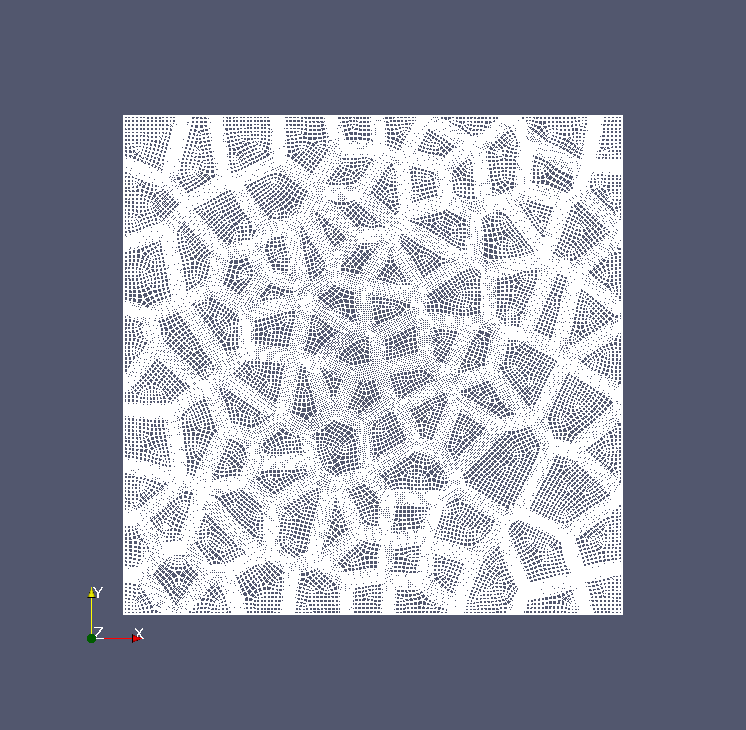
\includegraphics[trim = 0mm 0mm 0mm 0mm, clip,width=0.8\textwidth]{images/mesh_2D.png}
    \caption{The mesh used in Examples 1 and 2. Localization elements are
    used to mesh the grain boundaries indicated by the interface between grains 
    in different colors.}
    \label{fig:mesh}
\end{figure}

The mechanical and transport properties of the grain and grain boundaries for all numerical simulations are listed in Table \ref{tab.material.properties}. 
\begin{table}[h!]
\caption{\label{tab.material.properties}Transport and deformation properties of 21Cr-6Ni-9Mn austenitic stainless steel} \vspace{6pt}
\begin{center}
\begin{tabular}{|c|c|c|c|c|}
\hline
Physics &Property &Symbol &Value &Units\\
\hline
\multirow{5}{*}{Transport} & bulk pre-exponential factor &$D_{0}$ &5.4e-7 &$m^{2}/s$\\
\cline{2-5}
& boundary pre-exponential factor &$D_{0}$ &5.4e-4 to 5.4e-6 &$m^{2}/s$\\
\cline{2-5}
&activation energy &$Q$ &53.9e3 &$J/mol$\\
\cline{2-5}
&universal gas constant &$R$ &8.314 &$J/(mol K)$\\
\cline{2-5}
&temperature &$T$& 300 &$K$\\
\cline{2-5}
&lattice diffusivity &$D_{L}$ &2.2e-16 &${m}^2/s$\\
\cline{2-5}
&Avagadro's number&$N_{A}$ &6.0221e23 &$atoms/mol$\\
\cline{2-5}
&molar volume of metal&$V_{M}$& 7.116e-6 &${m}^3/mol$\\
\cline{2-5}
&partial molar volume of H&$V_{H}$ &2.0e-6 &${m}^3/mol$\\
\cline{2-5}
&atomic density of metal&$N_{L}$ &1.40e5 &$mol/m^{3}$\\
\cline{2-5}
&initial lattice concentration &$C_{L,0}$ &38.7 &$mol/m^{3}$\\
\cline{2-5}
&applied lattice concentration &$C_{L,app}$ &560 &$mol/m^{3}$\\
\cline{2-5}
&traps per defect &$\alpha$ &10 &$mol/mol$\\
\cline{2-5}
&power-law trapping parameter &$A$ &26.6 &$-$\\
\cline{2-5}
&power-law trapping parameter &$B$ &1.5 &$-$\\
\cline{2-5}
&power-law trapping parameter &$C$ &6.96 &$-$\\
\cline{2-5}
&baseline trap binding energy &$W_{B}$ &9.65e3 &$J/mol$\\
\cline{2-5}
&equilibrium constant &$K_{T}$ &47.9&$-$\\
\cline{2-5}
&equilibrium constant &$C_{T,0}$ &0.268&$mol/m^{3}$\\
\cline{2-5}
%\cline{2-4}
%&$c_{d}$ &9280 &$m/s$\\
%\cline{2-4}
%&$c_{s}$ &5620 &$m/s$\\
%\cline{2-4}
%&$c_{R}$ &5120 &$m/s$\\
\hline \multirow{5}{*}{Deformation}
&density &$\rho$ &7806 &$kg/m^{3}$ \\
\cline{2-5}
&Young's modulus &$E$ &197 &$G\!Pa$ \\
\cline{2-5}
&Poisson's ratio &$\nu$ &0.3 &$-$ \\
\cline{2-5}
&yield stress &$\sigma_{0}$ &590 &$M\!Pa$\\
\cline{2-5}
&hardening &$H$ &1227 &$G\!Pa$\\
\cline{2-5}
&hardening exponent &$m$ &0.563 &$-$\\
\cline{2-5}
\hline
\end{tabular}
\end{center}
\end{table}

\subsection{Numerical example 1: hydrogen flux in rigid micro-structure}
In We solved the hydrogen transport problem assuming that no deformation 
occurs during the transport process. As a result, the governing equation listed in \eqref{eq.hconservationref5} is reduced to the Fick's law with nonlinear diffusivity. 
Previously, coupling between grain boundary and bulk in polycrystalline nickel has been studied in
\citet{Jothi:2013}. In this study, The micropolycrystalline grain and grain boundaries are meshed with the same type of finite element.

Our main departure on the numerical treatment in this example is the usage of localization element.  

\subsection{Numerical example 2: hydrogen flux in micro-structure under a tension load}


Our main departure from the literature is threefold. First, .... localization element for both diffusion and displacement (JAY CAN UPDATE THIS LATER)

In this example, we examine the effect of elastic deformation on the hydrogen concentration.  For this simulation, we utilize a 3D bar that has a width and length of $1 \: \mu m$ and thickness of $0.1 \: \mu m$.  Additionally, plane strain is imposed such that the imposed displacements only change the length and width dimensions.  Displacement boundary conditions are imposed at the two opposite vertical edges.  The left end is restrained from motion, and the right end has a fixed velocity.  The hydrogen flux on the left end is increased linearly in time from $C_{L,0}$ until it reaches its final value $C_{L,app}$ while the hydrogen concentration on the right (displaced) end is fixed at the initial concentration (this configuration is shown in figure \ref{fig:DeformedConcentration}).  The displacement field and deformation gradient take the following form:
\begin{equation}
\label{eq.disp_defGrad_ex2} \boldsymbol{u} = 
\begin{bmatrix}
A t X_1 \\
B t X_2 \\
0 \\
\end{bmatrix}
, \indent
\boldsymbol{F} = 
\begin{bmatrix}
1 + A t & 0 & 0 \\
0 & 1 + B t & 0 \\
0 & 0 & 1 \\
\end{bmatrix}
\end{equation}
The elastic stored-energy function is computed assuming a Neo-Hookean material model of the following form:
\begin{equation}
\label{eq:neoHookeanEnergy}
W = \frac {1} {2} \kappa  \bigg [ \frac {1} {2} (J_e^2 - 1) - ln J_e \bigg ] + \frac {1} {2} \mu \bigg [ J_e^{-2/3} tr(\boldsymbol{b}_e) -3 \bigg]
\end{equation}
Where $\kappa$, $\mu$, $J_e$, and $\boldsymbol{b_e}$ are the bulk modulus, shear modulus, elastic jacobian, and elastic left stretch tensor, respectively.  With this material model, the Cauchy stress becomes
\begin{equation}
\label{eq:neoHookeanStress}
\boldsymbol{\sigma} = 2 J^{-1} \boldsymbol{F}_e \frac {\partial W} {\partial \boldsymbol{C}_e} \boldsymbol{F}_e^T = \frac {1} {2} \kappa \bigg [ J_e - J_e^{-1} \bigg] \boldsymbol{I} + J_e^{-5/3} \mu dev[\boldsymbol{b}_e]
\end{equation}
The constant $A$ in equation \ref{eq.disp_defGrad_ex2} is selected as $0.0005$ (assuming that the length dimension is in meters).  With the Neo-Hookean model shown above, the parameter $B$ is implicitly a function of the deformation along the $X1$ direction.  Since the imposed displacement field shown in equation \ref{eq.disp_defGrad_ex2} is linear, the strains (and therefore stresses) are constant, assuming a linear elastic material response.  This will simplify the expression in equation \ref{eq.hconservation3} by eliminating the pressure gradient term.  

\begin{figure}[H]
	\centering
	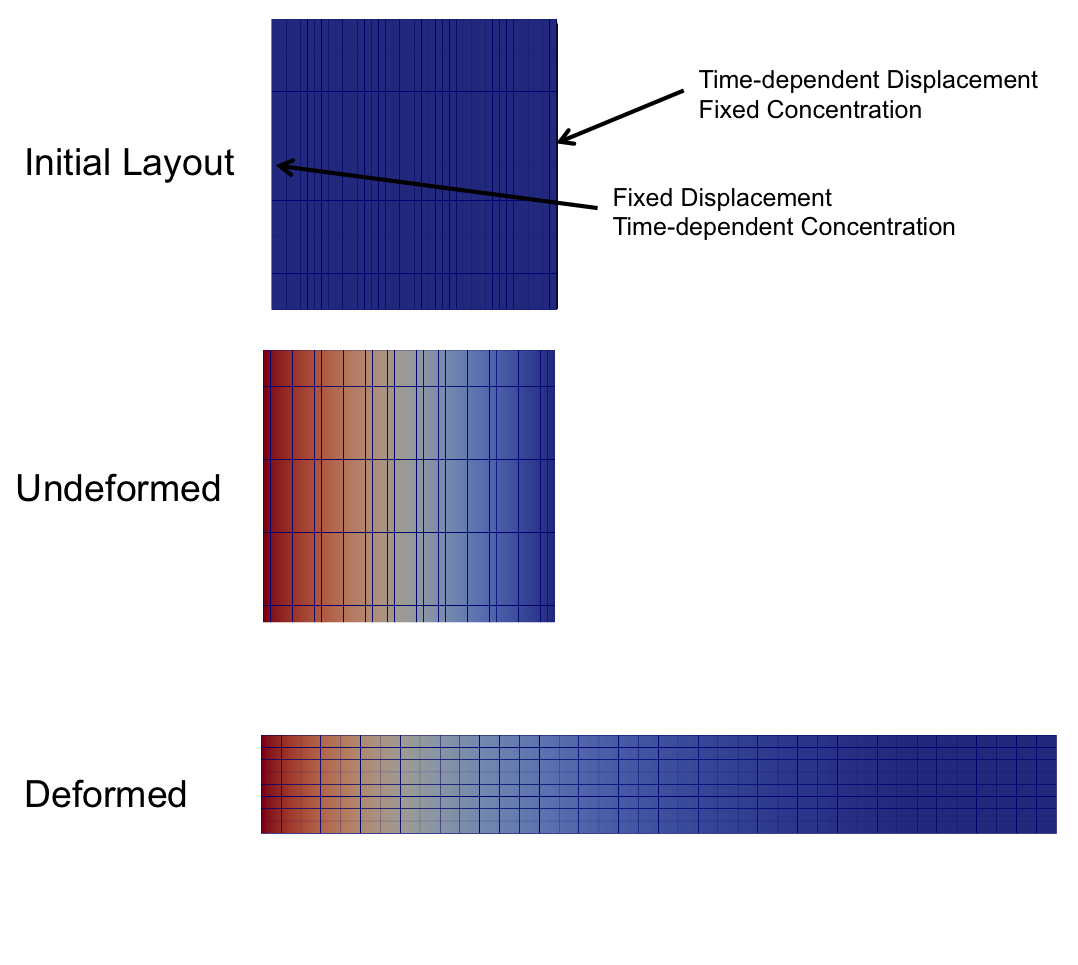
\includegraphics[trim = 0mm 0mm 0mm 0mm, clip,width=1.0\textwidth]{images/DeformedConcentration.png}
	\caption{A comparison of the hydrogen concentrations along the undeformed (top) and deformed (bottom) length of the bar.}
	\label{fig:DeformedConcentration}
\end{figure}

\begin{figure}[H]
	\centering
	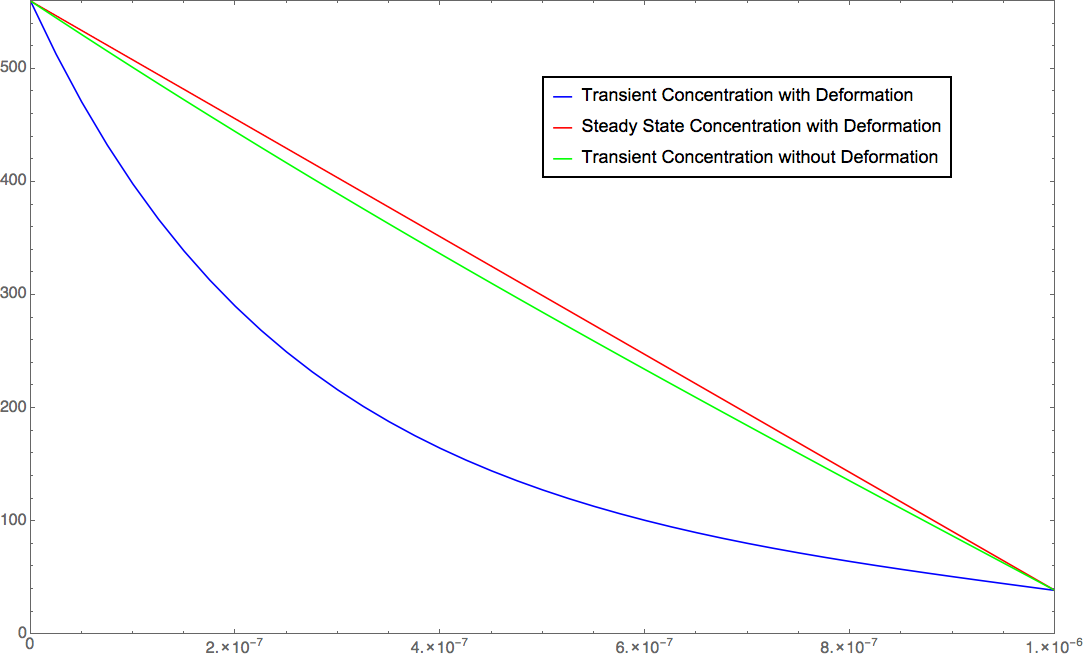
\includegraphics[trim = 0mm 0mm 0mm 0mm, clip,width=0.9\textwidth]{images/ConcentrationPlot.png}
	\caption{Comparison of the transient and steady state hydrogen concentration of the deformed bar (as a function of the initial position) to the transient hydrogen concentration of an undeformed bar}
	\label{fig:ConcentrationPlot}
\end{figure}


As shown in figures \ref{fig:DeformedConcentration} and \ref{fig:ConcentrationPlot}, the hydrogen concentration field in the current configuration after 10,000 time steps is nonlinear, as is expected since the PDE governing the dynamic transport of hydrogen molecules obeys Fick's second law.  Once the simulation reaches 10,000 time steps, the imposed displacement and concentration on the boundaries are held constant at their current values for the remainder of the simulation.  At 200,000 time steps, the concentration field diffuses and reaches steady state, as shown by the red curve in figure	 \ref{fig:ConcentrationPlot} (note that the steady-state solution produces a straight line).  In contrast, the transient concentration field in an undeformed bar after 10,000 time steps (green curve) nearly resembles the steady-state concentrations of the deformed bar.  The concentration distribution of the transient deformed bar exhibits a distinctively higher degree of nonlinearity than the undeformed bar.  This result illustrates the significance and importance of the pullback operation on the concentrations in the current configuration.  This pullback (via the inverse of the right stretch tensor, as expressed in equation \ref{eq.hconservationref5_1}) therefore plays a key role in coupling the chemical diffusion with the mechanical loading.
\subsection{Numerical example 3: hydrogen flux in K-field specimen}


%------------------ conclusion ----------------------
\section{Conclusion}

%\section{Acknowledgements}
%
%J.W.F. is grateful for the support of Sandia National Laboratories, operated by Sandia Corporation, a
%Lockheed Martin Company, for the United States Department of Energy
%under contract DE-AC04-94AL85000.

%------------------------ bibliography ----------------------
\clearpage
\bibliographystyle{elsart-harv_jwfoulk}
%\bibliographystyle{elsart-harv}

\bibliography{../../bibliography/fracture_mod,../../bibliography/fracture_exp,../../bibliography/HydrogenCoupling_stab}
%------------------------ bibliography ----------------------
%------------------------ appendices -----------------------
%
\appendix
\section{Stabilization proceedure}
\label{sec:appendixStab}
For stainless steel or other materials with very low diffusivity, the transient hydrogen
transport simulation may exhibits spurious oscillation if standard Galerkin method is
used without introducing proper stabilization. This spurious oscillation may exist
with or without boundary layer, and can lead to misleading, mesh dependent hydrogen profiles. Harari analyzed this numerous deficiency in \citep{Harari:2004} and found that spurious oscillation occurs in the linear transient diffusivity problem if the following condition holds, 
\begin{equation}
\label{eq:StabilityLimit} \frac{D^{*}}{D_{L}} < \frac{6 \vartheta \Delta t}{h^{2}}
\end{equation}
where $h$ is the mesh size, $\Delta t$ is the time step size and $\vartheta \in [0,1]$
is the integration parameter which leads to backward Euler scheme if $\vartheta = 1$
and forward Euler scheme if $\vartheta = 0$. One of the feasible cure to the
pathological mesh dependence is to introduce stabilization schemes such that
the spurious mode is eliminated from the numerical solutions without introducing
significant over-diffusion. Artificial diffusion,
lumped mass, Petrov-Galerkin, Galerkin least square, finite increment calculus and
projection based stabilization procedures are some of the commonly used
procedures available in finite element method literature \citep{Onate:2000,
Dohrmann:2004, Johnson:2009, Sun:2013}. 
In this study, we adopt an adaptive projection based stabilization procedure
originated in \citep{Sun:2013}. In this formulation,  a stabilization term is introduced into the residual of the weak
form of the transport equation \eqref{eq.hconservationref5}, i.e.,
\begin{equation}
\label{eq:stabilization2} R^{stab}(v, C_{L}) = \sum_{K \in \Omega}  \int_{K}  \Big( v  - \Pi (v)  \Big)  \gamma D^{*} \Big( C_{L} - \Pi (C_{L}) \Big)  dV
\end{equation}
$\Pi(\cdot)$ is a $L^{2}$ projection operator that projects $C_{L}$ onto a piecewise constant $\Pi (C_{L})$ and $\gamma$ is the stabilization parameter. One may think of the stabilization term in \eqref{eq:stabilization2} as a penalty that limits how much the data at one node affect the solution at all nodes, and therefore constrains spatial oscillations when near the hyperbolic limit with $D=0$ (note: in standard Galerkin method with consistent mass, the data at one node always affect all solution at all nodes even when $D=0$).

To illustrate this point and for the completeness of presentation, we briefly revisit the stabilized formulation here. Consider hydrogen transport in a 1D bar at which linearized transient diffusion neglecting the hydrostatic
stress term reads, 
\begin{equation}
\label{eq:perturbationP}  D \frac{ \partial^{2} C_{L} }{\partial x^{2}} =  \frac{\partial C_{L}}{\partial t},
\end{equation} 
where $D=D_{L}/D^{*}$. Equations taking the form of \eqref{eq:perturbationP} can be
discretized in time and that leads to a modified Helmholtz operator in
space \citep{Harari:2004}, which reads,
\begin{equation}
\label{eq:semidisform}
C_{L}^{n+1} + \vartheta  D \Delta t \frac{\partial^{2}}{\partial x^{2} }C_{L}^{n+1} = C_{L}^{n} - (1-\vartheta) D \Delta t \frac{\partial^{2}}{\partial x^{2}} C_{L}^{n} 
\end{equation}
where $C_{L}^{i}$ denotes the lattice concentration of hydrogen at $i$-th time step.
 Without introducing any boundary
conditions, \eqref{eq:semidisform} has an exact solution that reads
\citep{Harari:2004},
\begin{equation}
  \label{eq:FreeexactSol} 
  C_{L}(x) = \exp ( \pm x/\sqrt{\vartheta D \Delta t}) 
\end{equation}
Notice that the finite element approximate growth and decay rate of
the solution can be determined by assuming that $x_{A} = Ah$ such
that,
\begin{equation}
  \label{eq:approxgrow} 
  C_{L}^{A} = \exp ( \pm  (h/  (\sqrt{\vartheta D \Delta t})^{h} )^{A}
\end{equation}
where $\sqrt{\vartheta D \Delta t}^{h} $ is the approximate
growth/decay term in the finite element solution. Obviously the finite
element solution may exhibit spurious oscillations if $\sqrt{\vartheta
  D \Delta t}^{h}$ is complex valued, as pointed out in
\citep{Harari:2004}. 

To determine the range of the stabilization
parameters that prevent $\sqrt{\vartheta D \Delta t}^{h}$ being
complex valued, we consider a simple case in which piecewise-linear
finite elements are of uniform size $h$. As a result, we may construct
a three-node stencil via the standard Galerkin method, i.e.,
\begin{eqnarray}
\label{eq:standardGM}
 &-&C_{L}^{A-1} + 2 C_{L}^{A}  - C_{L}^{A-1} \nonumber \\ 
 &+& \frac{h^{2}}{6 \vartheta D\Delta t  }  \Large( C_{L}^{A-1} + 4 C_{L}^{A} + C_{L}^{A+1} \Large)  = 0  
\end{eqnarray}
Substituting the solution in \eqref{eq:approxgrow} leads to the following relation \citep{Harari:2004}, 
\begin{equation}
  \label{eq:Orgcoshbound} 
  \cosh \frac{h}{(\sqrt{\vartheta D \Delta t})^{h} }= \frac{ (1 + h^2/\vartheta D \Delta t) /3 }{ (1 - h^2/\vartheta D \Delta t) /6}
\end{equation}
By examining \eqref{eq:Orgcoshbound}, one may notice that the exponential growth
rate will become complex-valued if  \eqref{eq:StabilityLimit} is not hold. Now let us introduce the stabilziation term  \eqref{eq:stabilization2} into
\eqref{eq:semidisform}. By assembling the effective stiffness matrices
of the $L^{2}$ projection stabilization term, we obtain,
\begin{eqnarray}
\label{eq:L2correction}
 & -C_{L}^{A-1}  & + 2 C_{L}^{A}  - C_{L}^{A-1} \nonumber \\ 
 &+ \frac{h^{2}}{12 \vartheta c\Delta t  } & \Huge[ (2-\gamma)C_{L}^{A-1}  \nonumber \\
 & & + (8 +2\gamma) C_{L}^{A} + (2-\gamma) C_{L}^{A+1} \Huge]  = 0  
\end{eqnarray}
where $\gamma$ is the stabilization parameter for the pressure
projection term. 
To compute the stability bound for the $L^{2}$ projection stabilization,
we first apply \eqref{eq:approxgrow} into \eqref{eq:L2correction},
which leads to
\begin{equation}
  \label{eq:coshbound} 
  \cosh \frac{h}{(\sqrt{\vartheta D \Delta t})^{h} }= \frac{ (1 + h^2/\vartheta D \Delta t) ( 4 + \gamma)/6}{ (1 - h^2/\vartheta D \Delta t) ( 2 - \gamma)/12}
\end{equation}
The approximate growth/decay rate does not contain an imaginary part
if the hyperbolic cosine term is positive. Provided that $\gamma$ is positive, the stabilization parameter that eliminates
spurious oscillation can be determined from the denominator in the
right hand side of \eqref{eq:coshbound},
\begin{equation}
  \label{eq:stabL2bound} 
  \gamma > 2 -12 \frac{\vartheta D \Delta t}{h^{2}} > 0 
\end{equation}
Notice that the above formulation can be reduced to the
  classical 1D lumped mass case if $\gamma = 2$. In our implementation, 
  we employ the $L^{2}$ projection scheme and define $\gamma$ as
\begin{equation}
  \label{eq:arctang} 
  \gamma = (2 - 6 \frac{\vartheta D \Delta t}{h^{2}}) \Big(\frac{1}{2} + \frac{1}{2} \tanh( 2 - 12 \frac{\vartheta D \Delta t}{h^{2}}) \Big) 
\end{equation}
Notice that the term $1/2 + \tanh( 2 - 12 \frac{\vartheta D \Delta
  t}{h^{2}})/2 $ approaches zero if diffusivity is high and equal to 1
if diffusivity is low.  This treatment is to limit over-diffusion
caused by usage of the stabilization term as mentioned in
\citep{Sun:2013}. 

Finally, we also notice that  that stability of the steady state solution may also exhibit spurious oscillation if the P\'{e}clet number is less than one, i.e.,
\begin{equation}
\label{eq:Pnumber} P_{e}  = \frac{V_{H}}{RT} || \nabla_{\bs{X}}  S_{H} || h < 1
\end{equation} 
Nevertheless, since the condition listed in \eqref{eq:Pnumber} does not occur in our
numerical example for stainless steel due to the small molar volume, the
advection-dominated stabilization is not considered in this paper. Interested readers
may refer to \citep{Onate:2000} and \citep{Tezduyar:1986} for further details. 

\appendix
\section{Implementation in Albany}
\label{sec:appendixImplementation}
The fully coupled hydrogen transport  problem is implemented
in a problem solving environment called the Laboratory for Computational Mechanics
(LCM). LCM is an open-source computational mechanics environment
which utilizes the agile components code Albany \citep{Salinger:2010, Salinger:2013}
as its code base. Both Albany and the LCM are developed at Sandia
National Laboratories, and leverage strongly the open source
Trilinos project \citep{Heroux:2005}. This problem solving
environment employs a template-based generic programming approach
to fully integrate algorithms and technologies required to solve
large-scale problems in an object-oriented framework. This
approach offers several salient features over current
computational mechanics environments, including but not limited
to, rapid and flexible additions of physics and the automatic
propagation of derivatives. Here we provides a brief overview
of these features.

%\subsection{Evaluator Class}
 A typical numerical model consists of a description of a physical process
stemming from a governing equation or physical quantities whose values 
and properties depend on each others. For instance, in the hydrogen
transport problem defined in \eqref{eq.hconservation2}--\eqref{eq.hconservation5},
changes of temperature $T$ leads to change on the equilibrium constant $k_{T}$
and in return affects the trapped concentration $C_{T}$, the effective diffusion
constant $D^{*}$ and the diffusion coefficient $D_{L}$ and therefore affect how 
lattice concentration of hydrogen distribute in the metal. 

If the weak form of the governing equation \eqref{eq.hconservation5} is 
consistently linearized, as in the fully implicit schemes available 
in the literature, then this 
hierarchical dependence must be taken into account via the chain rules. 
While deriving the tangents is certainly not a conceptually difficult task, 
it is otherwise a time-consuming process that requires 
substantial effort . Moreover, if any changes in the formulation leads to changes in 
the hierarchical structure of mathematical expressions, then the derivations of the consistent linearization must
start from scratch. 

In Albany, the agile components code we adopted to implement the hydrogen
transport model,  physical quantities, such as the equilibrium constant and the
diffusion coefficient, are programmed as C++ templates called \emph{evaluators}.
The hierarchical dependence of these physical quantities are recorded. 
This hierarchical structure of the evaluators can be used to obtain partial, total,
and directional derivatives via automatic differentiation tool available in 
Trillions. With the ability to automatically compute derivatives, collection of 
evaluators can be used to assembly the weak form. The consistent linearization
is done without directly implementing the expression of linearized
residuals of the field equations. 

Furthermore, usage of evaluators also make it
easier to debug, as the hierarchy of physical quantities can be easily visualized
as directed graph as shown in Figure \ref{fig:graph}. 
\begin{figure}[h!]
%  \centering
%    \includegraphics[trim = 0mm 0mm 0mm 0mm, clip,width=0.99\textwidth]{graph.pdf}
%    \caption{Directed graph that represents the weak form of the fully coupled
%    deformation-diffusion problem.}
%    \label{fig:graph}
\end{figure}
Interested readers please refer to \citep{Salinger:2010, Pawlowski:2012a, Pawlowski:2012b, Salinger:2013, Sun:2013}
for further detail on how multiphysics boundary value problems
are implemented in Albany. 

\end{document}
%

